\documentclass[12pt,a4paper]{article}
\usepackage[legalpaper, portrait, margin=2cm]{geometry}
\usepackage[portuguese]{babel}
\usepackage[utf8]{inputenc}
\usepackage{fancyhdr}
\usepackage{graphicx}
\usepackage{hyperref}
\usepackage{indentfirst}
\usepackage{listings}
\usepackage{xcolor}

\graphicspath{ {./} }
\hypersetup{
  colorlinks=true,
  linkcolor=blue,
  filecolor=magenta,
  urlcolor=blue,
  citecolor=blue,
  pdftitle={Exercício 8 - Projeto Computacional PE 2022/2023 LEIC-A},
  pdfpagemode=FullScreen,
}

\pagenumbering{gobble}
\pagestyle{fancy}
\fancyhf{}
\rhead{Grupo \textbf{11}}
\lhead{Exercício 8 - Projeto Computacional PE 2022/2023 LEIC-A}
\cfoot{Gonçalo Bárias (103124), Raquel Braunschweig (102624) e Vasco Paisana (102533)}

\renewcommand{\footrulewidth}{0.2pt}

\renewcommand{\labelitemii}{$\circ$}
\renewcommand{\labelitemiii}{$\diamond$}

\definecolor{codegreen}{rgb}{0,0.6,0}
\definecolor{codegray}{rgb}{0.3,0.3,0.3}
\definecolor{codepurple}{rgb}{0.58,0,0.82}

\lstdefinestyle{mystyle}{
  commentstyle=\color{codegreen},
  numberstyle=\tiny\color{codegray},
  % keywordstyle=\color{magenta},
  % stringstyle=\color{codepurple},
  basicstyle=\ttfamily\footnotesize, breakatwhitespace=false, breaklines=true,
  captionpos=b, keepspaces=true, numbers=left, numbersep=5pt, showspaces=false,
  showstringspaces=false, showtabs=false, tabsize=2 } \lstset{style=mystyle}

\begin{document}

% Introdução sobre o exercício em questão
O objetivo deste exercício é comparar valores gerados e ordenados por ordem crescente de uma distribuição cauchy com os
quantis de probabilidade $\frac{i}{195}, i = 1,…,194$ dessa população e de uma população normal de valor esperado
$\mu = 3.8$ e variância $\sigma^{2} = 4$.
Para tal, recorreu-se ao seguinte trecho de código em \texttt{R}:

\quad

% Código em R para resolver o exercício
\begin{lstlisting}[language=R]
SEED <- 1657
SAMPLE_SIZE <- 194
CAUCHY_LOCALIZATION <- 3.2
CAUCHY_SCALE <- 1.2
NORMAL_EXPECTED <- 3.8
NORMAL_VARIANCE <- 4
set.seed(SEED)

cauchy_sample <- rcauchy(SAMPLE_SIZE, CAUCHY_LOCALIZATION, CAUCHY_SCALE)

prob_quantiles <- seq(1 / 195, 194 / 195, by = 1 / 195)
cauchy_quantiles <- quantile(cauchy_sample, probs = prob_quantiles)
normal_quantiles <- qnorm(prob_quantiles, mean = NORMAL_EXPECTED, sd = sqrt(NORMAL_VARIANCE))

sorted_cauchy_sample <- sort(cauchy_sample)

plot(sorted_cauchy_sample, normal_quantiles, main = "QQ Plot: Valores Cauchy Gerados (Ordenados) vs Quantis de Probabilidade",
     xlab = "Valores Cauchy Gerados (Ordenados)", ylab = "Quantis de Probabilidade",
     xlim = range(sorted_cauchy_sample), ylim = range(normal_quantiles, cauchy_quantiles))
points(sorted_cauchy_sample, cauchy_quantiles, col = "#f8766d", pch = 19)
points(sorted_cauchy_sample, normal_quantiles, col = "#00bfc4", pch = 19)
abline(0, 1, col = "black", lty = 2)
legend("topleft", legend = c("Normal", "Cauchy", "y = x"),
       col = c("#00bfc4", "#f8766d", "black"), pch = c(19, 19, NA), lty = c(NA, NA, 2))
\end{lstlisting}

\quad

% Gráfico para resolver o exercício
\begin{figure}[h]
  \centering
  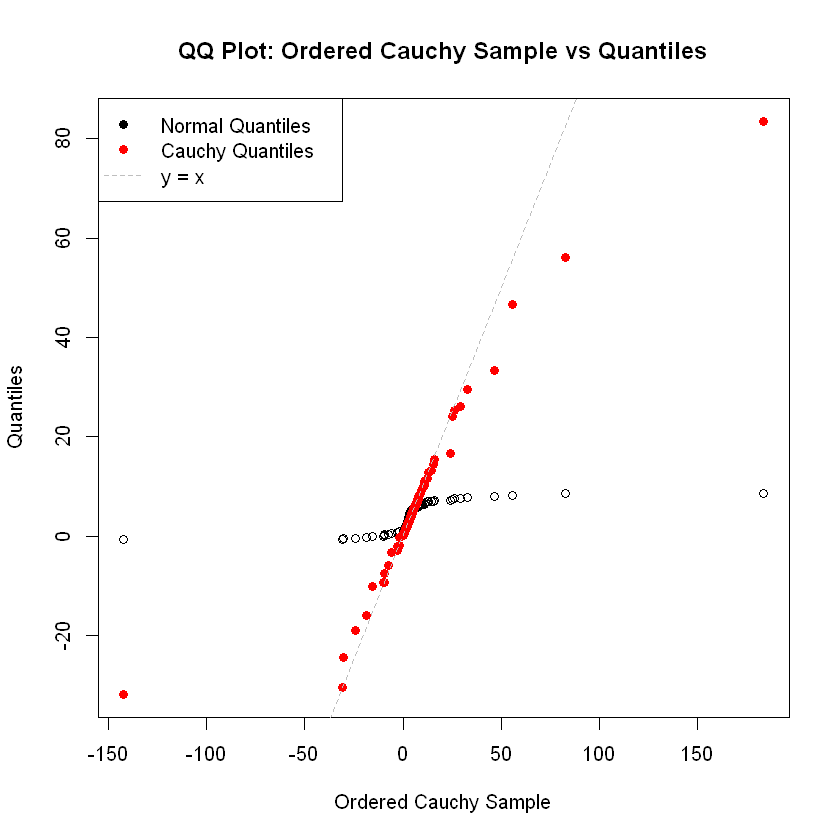
\includegraphics[scale = 0.77]{./ex08.png}
\end{figure}

\end{document}
